% Intended LaTeX compiler: pdflatex
\documentclass[11pt]{article}
\usepackage[utf8]{inputenc}
\usepackage[T1]{fontenc}
\usepackage{graphicx}
\usepackage{longtable}
\usepackage{wrapfig}
\usepackage{rotating}
\usepackage[normalem]{ulem}
\usepackage{amsmath}
\usepackage{amssymb}
\usepackage{capt-of}
\usepackage{hyperref}
\author{Construção de compiladores I}
\date{}
\title{Interpretadores}
\hypersetup{
 pdfauthor={Construção de compiladores I},
 pdftitle={Interpretadores},
 pdfkeywords={},
 pdfsubject={},
 pdfcreator={Emacs 28.2 (Org mode 9.7)}, 
 pdflang={English}}
\begin{document}

\maketitle
\section*{Objetivos}
\label{sec:org5383b56}

\subsection*{Objetivos}
\label{sec:org54f5c16}

\begin{itemize}
\item Apresentar o conceito de semântica operacional para especificar interpretadores.

\item Mostrar a equivalência entre definições semântica e implementação de interpretadores.
\end{itemize}
\section*{Introdução}
\label{sec:org3732cf4}

\subsection*{Introdução}
\label{sec:orgad9eedc}

\begin{itemize}
\item Nas aulas anteriores, vimos como construir a árvore de sintaxe abstrata a partir do texto do programa.
\begin{itemize}
\item Análise léxica e sintática
\end{itemize}
\end{itemize}
\subsection*{Introdução}
\label{sec:org46c8c3d}

\begin{itemize}
\item A partir da árvore de sintaxe abstrata, podemos:
\begin{itemize}
\item Fazer análise semântica.
\item Interpretar o código.
\item Gerar código
\end{itemize}
\end{itemize}
\subsection*{Introdução}
\label{sec:org75d987a}

\begin{itemize}
\item Antes de lidar com a análise semântica, vamos estudar sobre como construir intepretadores.
\begin{itemize}
\item Motivo: tornar evidente a necessidade da análise semântica.
\end{itemize}
\end{itemize}
\section*{Noções de semântica}
\label{sec:org228be1c}

\subsection*{Noções de semântica}
\label{sec:org5a36c98}

\begin{itemize}
\item Semântica formal: estudo de formalismos matemáticos para determinar o significado de programas.

\item Três abordagens principais: denotacional, axiomática e operacional.
\end{itemize}
\subsection*{Noções de semântica}
\label{sec:org4ac8457}

\begin{itemize}
\item Semântica denotacional.
\begin{itemize}
\item Modelar o significado do programa usando funções e domínios semânticos.
\item Vantagens: composicionalidade
\item Desvantagens: difícil modelar estado.
\end{itemize}
\end{itemize}
\subsection*{Noções de semântica}
\label{sec:org1955944}

\begin{itemize}
\item Semântica axiomática.
\begin{itemize}
\item Significado de um programa é o que pode ser provado sobre ele.
\item Utilizada para demonstrar propriedades de um programa.
\end{itemize}
\end{itemize}
\subsection*{Noções de semântica}
\label{sec:orga7abb8e}

\begin{itemize}
\item Semântica operacional.
\begin{itemize}
\item Semântica de programas expressa por meio de relações.
\item Dois estilos: big-step e small-step
\end{itemize}
\end{itemize}
\subsection*{Noções de semântica}
\label{sec:orgc30a768}

\begin{itemize}
\item Semântica big-step
\begin{itemize}
\item Definição como relações entre programas e seu resultado.
\item Associa um programa completo e seu respectivo resultado.
\end{itemize}
\item Ideal para especificar interpretadores.
\end{itemize}
\subsection*{Noções de semântica}
\label{sec:orgaf28c7d}

\begin{itemize}
\item Semântica small-step
\begin{itemize}
\item Definição como relações que mostram a execução passo-a-passo.
\end{itemize}

\item Útil para especificar provas.
\end{itemize}
\subsection*{Noções de semântica}
\label{sec:orgb67d048}

\begin{itemize}
\item Nosso foco no curso será no uso de semântica operacional big-step.

\item Porém, vamos mostrar a diferença entre big and small-step, usando uma linguagem simples e sua semântica.
\end{itemize}
\subsection*{Noções de semântica}
\label{sec:orgd569163}

\begin{itemize}
\item Linguagem considerada:
\end{itemize}

\begin{array}{lcl}
e & \to & n \,|\, e + e \,|\, e * e\\
\end{array}
\subsection*{Noções de semântica}
\label{sec:org27d7af9}

\begin{itemize}
\item Semântica big-step
\end{itemize}

\begin{center}
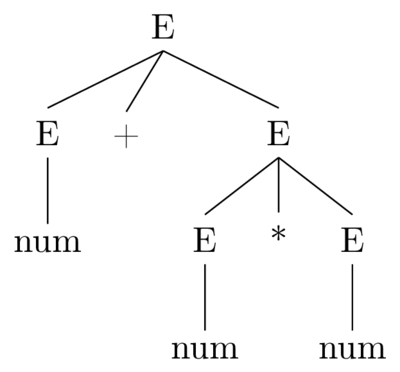
\includegraphics[width=.9\linewidth]{./imgs/image1.png}
\end{center}
\subsection*{Noções de semântica}
\label{sec:orgb8cd2cf}

\begin{itemize}
\item Semântica small-step
\end{itemize}

\begin{center}
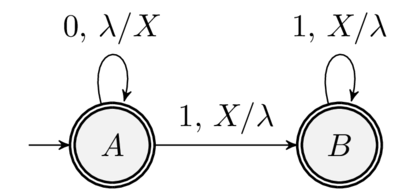
\includegraphics[width=.9\linewidth]{./imgs/image2.png}
\end{center}
\section*{Implementação}
\label{sec:orgb865781}

\subsection*{Implementação}
\label{sec:org3af3099}

\begin{itemize}
\item Sintaxe em Haskell
\end{itemize}

\begin{verbatim}
data Exp
  = Const Int
  | Exp :+: Exp
  | Exp :*: Exp
  deriving Show

newtype Value = VInt Int deriving Show
\end{verbatim}
\subsection*{Implementação}
\label{sec:orgf164b47}

\begin{itemize}
\item Semântica big-step
\end{itemize}

\begin{verbatim}
bigStep :: Exp -> Value
bigStep (Const n) = VInt n
bigStep (e1 :+: e2)
  = case (bigStep e1, bigStep e2) of
      (VInt n1, VInt n2) -> VInt (n1 + n2)
bigStep (e1 :*: e2)
  = case (bigStep e1, bigStep e2) of
      (VInt n1, VInt n2) -> VInt (n1 * n2)
\end{verbatim}
\subsection*{Implementação}
\label{sec:org17348bd}

\begin{itemize}
\item Semântica small-step
\end{itemize}

\begin{verbatim}
step :: Exp -> [Exp]
step (Const _) = []
step ((Const n1) :+: (Const n2))
  = [Const $ n1 + n2]
step ((Const n1) :*: (Const n2))
  = [Const $ n1 * n2]
step (e1 :+: e2)
  = [e1' :+: e2 | e1' <- step e1] ++
    [e1 :+: e2' | e2' <- step e2]
step (e1 :*: e2)
  = [e1' :*: e2 | e1' <- step e1] ++
    [e1 :*: e2' | e2' <- step e2]
\end{verbatim}
\subsection*{Implementação}
\label{sec:orgc49b35a}

\begin{itemize}
\item Semântica small-step
\end{itemize}

\begin{verbatim}
data Tree a = Node a [Tree a] deriving Show

multiStep :: Exp -> Tree Exp
multiStep e = Node e [multiStep e' | e' <- step e]
\end{verbatim}
\section*{Concluindo}
\label{sec:org783d2a9}

\subsection*{Concluindo}
\label{sec:org0956a9c}

\begin{itemize}
\item Nesta aula apresentamos uma introdução à construção de interpretadores e
semântica formal.

\item Próximas aulas: interpretadores para linguagens imperativas.
\end{itemize}
\section*{Exercícios}
\label{sec:org53f1a64}

\subsection*{Exercícios}
\label{sec:orgc04a765}

\begin{itemize}
\item Construa um analisador sintático para o código de exemplo para produzir um
interpretador completo para a linguagem de expressões.
\end{itemize}
\end{document}
